\documentclass[10pt,conference,compsocconf]{IEEEtran}

%\usepackage{times}
%\usepackage{balance}
\usepackage{amsmath}
\usepackage{url}
\usepackage{graphicx}	% For figure environment
\usepackage{color}
\usepackage{breqn}

\begin{document}
	\title{United We Stand:\\ Combinations for Collaborative Filtering}
	
	\author{
		\IEEEauthorblockN{Mariyana Koleva}
		\IEEEauthorblockA{
			ETH Zurich\\
			Switzerland\\
			Email: kolevam@student.ethz.ch} 
		\and
		\IEEEauthorblockN{Karim Labib}
		\IEEEauthorblockA{
			ETH Zurich\\
			Switzerland\\
			Email: labibk@student.ethz.ch} 
		\and
		\IEEEauthorblockN{Jo\~{a}o Louren\c{c}o Ribeiro}
		\IEEEauthorblockA{
			ETH Zurich\\
			Switzerland\\
			Email: ljoao@student.ethz.ch} 
	}
	
	\maketitle
	
	\begin{abstract}
		Collaborative filtering consists of making predictions about some unknown preferences of a user based on  available data from a set of users. There exist several philosophies for tackling this problem, and algorithms from each different philosophy pick up distinct properties from the data. In this paper, we study whether we can obtain better predictions by combining results from algorithms based on two different approaches: latent-factor and neighborhood-based models. We also study the effect of adding a learning rate heuristic to some algorithms.
	\end{abstract}
	
	\section{Introduction}
	
	Recommender systems have gained popularity in the last decade due to their immediate market applications. The huge selection of products allow online retailers to attract a wide-range of clients. However, it also means that users can no longer be expected to browse through everything available until they find what they like the most. Good recommendations are thus key for many leading online ventures, notably Netflix \cite{amatriain2012netflix}, and Amazon \cite{linden2003amazon}.
	
	In this paper, we concentrate on the collaborative filtering approach to recommender systems, which relies on previous user experiences (ratings), rather than predefined user profiles. Our problem and data are largely based on the Netflix challenge \cite{SMH07}, \cite{Koren09matrixfactorization}, \cite{funk2011netflix}.
	
	Our main contributions are two-fold. We first combine latent factor models and neighbourhood models to produce a robust recommender system which optimizes the Root Mean Squared Error (RMSE) of 1176953 predicted ratings from \textbf{Base score} to \textbf{Best score without BD}. Secondly, we show that the addition of a more complex learning rate heuristic on two latent factor models improves the score significantly, to \textbf{best score}. 
	
	In Section \ref{sec:models} we describe the idea and the implementation of our systems. We present the results from the local evaluation of the models and from the validation set on Kaggle in Section \ref{sec:results}. Finally, in Section \ref{sec:conclusions} we draw conclusions from the analysis of the various methods and reported results.
	
	
	\section{Models and Methods}
	\label{sec:models}
	The dataset on which the work was based is a collection of \emph{(user, movie, rating)} tuples. For training, we have 1176953 ratings available. The online evaluation on Kaggle is performed on another 1176953 ratings. We were able to see the prediction accuracy on 50\% of the online dataset, and we aimed to improve it.
	\subsection{Data Model}
	
	The provided dataset can be seen as an $N\times M$ matrix, with $N$ being the number of users ($N=~10000$), and $M$ the number of movies ($M=1000$). If every user had rated every movie, the matrix would have $10^7$ entries. However, in our case, the matrix is quite sparse. From here stems the difficulty of the problem -- we attempt to predict more than a million ratings based on a representative subset. 
	
	There are two main views which yield different methods for tackling this problem.
	
	\subsubsection*{\textbf{Latent factor models}} 
	
	%{\color{red} Modify because of RBM} This approach tries to explain the ratings as influenced by a set of unknown (latent) factors. Both users and items can be characterized by these latent factors and they are represented as low-dimensional feature vectors in this latent feature space. The rating of a movie is approximated by the dot product between the user and movie feature vectors.
	%
	%The different methods then aim to infer the underlying movie and user feature vectors from the available ratings, most successfully through matrix factorization techniques and approximations. We discuss Singular Value Decomposition and Stochastic Gradient Descent as particular examples of methods which follow this approach.
	%
	%We also discuss another latent factor model which is based on a different philosophy.
	
	These models attempt to explain movie ratings by users as being influenced by a set of unknown (also called \emph{latent}) factors.
	
	One approach characterizes users and movies by low-dimensional feature vectors in a latent feature space. The missing rating of a given movie by a given user is modeled as the dot product between the corresponding user and movie feature vectors. As  examples of this approach, we discuss Singular Value Decomposition (SVD) and Stochastic Gradient Descent (SGD).
	
	It is also possible to predict missing ratings through neural networks which are composed by visible and latent units. We focus on Restricted Boltzmann Machines (RBM).
	
	
	\subsubsection*{\textbf{Neighborhood-based models}} 
	Another approach is to view the ratings as features of either the users (user-based) or the movies (item-based). In the user-based (item-based) perspective, we predict a missing rating of movie $j$ by user $i$ from the ratings of similar users (movies) to $i$ ($j$), according to some distance function. We review implementations of both these ideas: user-based and item-based $k$-Nearest Neighbors (kNN).
	
%	Another approach is to view the ratings as features of either the users (user-based) or the movies (item-based). In the former case, a user is represented as a sparse feature vector of their ratings and we would base our prediction on other users who have rated those movies similarly. In the latter scenario, we would use the similarity between the new movie and the movies already rated by  to estimate the new rating. Each movie is a feature vector of all users' ratings. We review an implementation of both ideas in the next subsection.
	
	\subsection{Algorithms}
	We used three latent-factor and two neighborhood-based algorithms:
	
	\subsubsection*{\textbf{SVD}} For this algorithm, we view the rating matrix as the product of a user matrix and a movie matrix, which are both on the latent factors' feature space. SVD is a natural method for performing this decomposition \cite{Koren09matrixfactorization}. The main issue we face is that SVD works on full matrices only. Hence, we need to impute the missing values before we can proceed. If rating $r_{ij}$ is missing, we impute the value $\lambda \textnormal{AvgUser}[i] + (1 - \lambda) \textnormal{AvgFilm}[j]$, where $\lambda \in [0,1]$, and $\textnormal{AvgUser}[i]$ and $\textnormal{AvgFilm}[j]$ are the average ratings of user $i$ and movie $j$, respectively. 
	
	%Imputation in general introduces noise and leads to sup-optimal results \cite{Koren09matrixfactorization}. We hope to minimize the noise and over-fitting by looking for a low-rank ($k$) approximation of the rating matrix.
	
%	\begin{equation}
%	r_{ij}= \lambda \textnormal{AvgUser}[i] + (1 - \lambda) \textnormal{AvgFilm}[j],
%	\label{eq:imputation}
%	\end{equation}
	
	We experimented with different values for $\lambda$ and numbers of latent features. We concluded that the lowest RMSE on a probe set was accomplished using 13 features and $\lambda = 0.25$.
	
	Nevertheless, we expect the results achieved with SVD to be suboptimal due to the large number of missing values, and the inaccuracy introduced by the imputation of those values. We use this algorithm as a baseline and we try to improve on it.
	
	\subsubsection*{\textbf{SGD}} Instead of using the standard SVD, which requires a full matrix, we can use only the available ratings in a Stochastic Gradient Descent method. The regularized (to avoid over-fitting) objective function to minimize is as follows:
	
	\begin{equation}
	\begin{split}
	\min_{p,q,b_u,b_m} \sum_{(i,j) \in T} &(r_{ij} - (b_u(i) + b_m(j) + p_i^T \cdot q_j))^2 \\ &+ \lambda(\lVert p_i \rVert^2 + \lVert q_j \rVert^2 + b_u(i)^2 + b_m(j)^2).
	\end{split}
	\end{equation}
	
	$T$ is the set of observed ratings (pairs $(i,j)$ of user $i$ rating movie $j$), $r_{ij}$ is the known rating of user $i$ to movie $j$, and $b_u$ and $b_m$ are the bias vectors of users and movies respectively. It has been pointed out in \cite{Koren09matrixfactorization} that the bias vectors lead to higher accuracy. Intuitively, these biases help us as some user tend to consistently rate higher than others. In order to predict an unknown rating of user $i$ to movie $j$ we compute $r_{pred} = b_u(i) + b_m(j) + p_i^T\cdot q_j$.
	The parameters are modified during the algorithm by looping through all ratings in the training set for several epochs. The learning rules are
	\begin{equation}
	\begin{split}
	p_i &\leftarrow p_i + \gamma(e_{ij}q_j - \lambda p_i) \\
	q_j &\leftarrow q_j + \gamma(e_{ij}p_i - \lambda q_j) \\
	b_u(i) &\leftarrow \gamma(e_{ij} - \lambda b_u(i)) \\
	b_m(j) &\leftarrow \gamma(e_{ij} - \lambda b_m(j)).
	\end{split}
	\end{equation}
	The algorithm was very sensitive to hyper-parameters, so those were optimized on both a local validation set and the online Kaggle score.
	
	\subsubsection*{\textbf{Restricted Boltzmann Machines (RBM's)}}
	
	RBM's are neural networks consisting of a layer of visible units and a layer of hidden units. Each unit has a stochastic binary random variable associated with it. There may be undirected connections between hidden and visible units, but no hidden-hidden or visible-visible connections are allowed. These networks are a restricted version of Boltzmann machines (hence the name), introduced in \cite{AHS85}.
	
	Recently, RBM's have found applications in collaborative filtering, as illustrated in \cite{SMH07}. A very nice overview of RBM's for collaborative filtering can be found in \cite{L10}. Our approach is based on these two works, although there are some differences.
	
	We first build an RBM with 5000 visible units $v^k_i$, for $k\in\{1,\dots,5\}$ and $i\in\{1,\dots,1000\}$, and $L$ hidden units $h_1,\dots, h_L$, where $L$ is a hyper-parameter of the algorithm. Furthermore, for each hidden unit $h_j$ we add connections to every visible unit $v^k_i$. Each connection between $h_j$ and $v^k_i$ has an associated weight $W^k_{ij}$. Each hidden unit $h_j$ has an associated bias $b_j$ and each visible unit $v^k_i$ has an associated bias $b^k_i$. Finally, each unit can be in state 0 or 1.
	
	The probability that a given unit is turned on (i.e. its associated state is 1) is a logistic function of the states of the units it is connected to. 
	
%	In our case we have
%	\begin{equation}
%	\begin{split}
%	p(v^k_i=1|h)&=\frac{\exp(b^k_i+\sum_{j=1}^L h_jW^k_{ij})}{\sum_{l=1}^{5}\exp(b^l_i+\sum_{j=1}^{L}h_jW^l_{ij})}\\
%	p(h_j=1|V)&=\frac{1}{1+\exp(-b_j-\sum_{i=1}^{1000}\sum_{k=1}^{5}v^k_iW^k_{ij})}.
%	\end{split}
%	\end{equation}
	
	To train our RBM, we divide the users into small batches. For each user $u$ in a batch, we encode its ratings as follows: $v^k_i=1$ if and only if user $u$ gave rating $k$ to movie $i$. After going through each batch, we update the weights and biases. We omit a detailed description of the training procedure and of the learning rules, which can be found in \cite{L10}. Some quantities needed for the updates are hard to compute exactly, but they can be approximated efficiently via Gibbs sampling (see \cite{H02}). In our algorithm we use a single step of Gibbs sampling. According to \cite{L10}, this yields a good approximation already.
	
%	We then compute $p_j=p(h_j=1|V)$ when $V=\{v^k_i\}$ is set according to each of the users in the batch, and record $v^k_i$ and $p_j$ for each triple $(i,j,k)$.
%	The learning rules are
%	
%	\begin{equation}
%	\begin{split}
%	W^k_{ij} &\leftarrow W^k_{ij} + \gamma(<v^k_ih_j>^+-<v^k_ih_j>^-)\\
%	b^k_i &\leftarrow b^k_i + \gamma(<v^k_i>^+-<v^k_i>^-)\\
%	b_j &\leftarrow b_j + \gamma(<h_j>^+-<h_j>^-),
%	\end{split}
%	\end{equation}
%	where $\gamma$ is the learning rate, $<v^k_ih_j>^+$ is the average (over all users in the batch) of $v^k_i\cdot p_j$, $<v^k_i>^+$ is the average of $v^k_i$ and $<h_j>^+$ is the average of $p_j$. Furthermore, $<v^k_i>^-$ and analogous quantities correspond to averaged probabilities of finding the corresponding units turned on simultaneously when the neural network is running at equilibrium. 
	
	Note that we train only a single RBM. In \cite{SMH07}, the method presented consists of building a different RBM for each user, which all share the same weights and biases. In particular, they keep only connections from hidden units to visible units corresponding to observed ratings of a particular user.
	
	The prediction algorithm is the same in our method and in \cite{SMH07} and \cite{L10}. Namely, for a fixed user $u$, we set $v^k_i=1$ if and only if user $u$ ranked movie $i$ with rating $k$. We then compute $\hat{p}_j=p(h_j=1|V)$ for $j=1,\dots, L$. If we want to predict the rating of movie $i$, we compute
	\begin{equation}
	p(v^k_i=1|\hat{p})=\frac{\exp(b^k_i+\sum_{j=1}^L \hat{p}_jW^k_{ij})}{\sum_{l=1}^{5}\exp(b^l_i+\sum_{j=1}^{L}\hat{p}_jW^l_{ij})},
	\end{equation}
	for $k=1,\dots, 5$. This yields a probability distribution over the possible ratings for movie $i$. Our prediction is the expected value of this distribution, $\sum_{k=1}^{5}k\cdot p(v^k_i=1|\hat{p})$.
	
	We make use of the built-in BernoulliRBM algorithm in the \emph{sklearn} Python library to create our RBM and train it. Furthermore, we modified the source code to add a heuristic for the learning rate of the RBM, which improved its performance.
	
	\subsubsection*{\textbf{User-based $k$-Nearest Neighbors}} User based neighbourhood algorithms consist of two steps. First, the algorithm computes the similarity between different users through some similarity measure. Second, to predict the rating of user $u$ for a particular movie $m$, the ratings of the most similar $k$ users who have rated movie $m$ are aggregated to estimate the required rating. The similarity measure, which according to \cite{L10} was found to be the most accurate, was the Pearson correlation measure. We denote the Pearson correlation between two users $u_1$ and $u_2$ by $w(u_1, u_2)$ and it is calculated as follows:
	\begin{equation} \label{eqn:pearson}
	\frac{\sum_{j \in C} (R(u_1, j) - \overline{R}_C(u_1))\cdot(R(u_2, j) - \overline{R}_C(u_2))}{\sqrt{\sum_{j \in C} (R(u_1, j) - \overline{R}_C(u_1))^2} \sqrt{\sum_{j \in C} (R(u_2, j) - \overline{R}_C(u_2))^2}},
	\end{equation}
	
	where $C$ is the set of co-rated items between users $u_1$ and $u_2$, $R(u,j)$ is the rating of user $u$ to movie $j$, and $\overline{R}_C(u)$ is the average rating of user $u$ on the set of movies $C$. The higher the correlation, the more similar the two users. This measure can be shown \cite{L10} to be equivalent to the cosine based similarity of the centered rating matrix (averages of users are subtracted from the corresponding ratings). This allows for easier and faster computation of correlation between every pair of users using \emph{sklearn}. The best $k$ was chosen by calculating the error of the algorithm on a validation set for different values of $k$. Finally, to predict the unknown rating of a user $u$ for a particular movie $i$, we compute an averaged weighted sum of the ratings of the $k$ nearest neighbors to user $u$ as follows:
	\begin{equation} \label{eqn:predict_user_based}
	R(u,i) = \overline{R}(u) + \frac{\sum_{u_k \in N(u)} w(u,u_k)(R(u_k,i) - \overline{R}(u_k))}{\sum_{u_k \in N(u)} w(u,u_k)},
	\end{equation}
	where $N(u)$ is the set of the $k$ most similar users who rated item $i$.
	\\
	
	\subsubsection*{\textbf{Item-based $k$-Nearest Neighbors}}  For this algorithm, we consider neighborhoods of movies, instead of users. Computing the neighborhood of a movie and the predictions can be done in an analogous fashion to user-based kNN. Again, we make use of the Pearson correlation measure. The size of the neighborhood of a movie is a hyper-parameter that is optimally chosen using a local validation set.
	
%	The set of users who rated movies $i$ and $j$ are used to measure as two vectors and the correlation is measured between them in a similar fashion as shown in equation (\ref{eqn:pearson}). in order to predict the rating of user $u$ for movie $i$, This is computed as follows:
%	\begin{equation}
%	R(u,i) = \overline{R}(i) + \frac{\sum_{j \in k_R(u)} w(i,j)(R(u,j) - \overline{R}(j))}{\sum_{j \in k_R(u)} w(i,j)},
%	\end{equation}
%	where $\overline{R}(i)$ is the average rating of movie $i$,  $k_R(u)$ is a set of movies for which we know the rating of user $u$, and $w(i,j)$ is the similarity measure of movie $i$ and movie $j$.
	
	\subsection{The bold driver heuristic} 
	A significant improvement to the running time and efficiency of our algorithm came from incorporating the bold driver heuristic for the learning rate in both SGD and RBM. This technique works as follows: Suppose we start with learning rate $\lambda$. After each epoch we compute the current error on the validation set and compare it with the error of the previous epoch. If the error increased from one epoch to the other, we decrease $\lambda$ to $d\lambda$, where $d\in[0,1]$. On the other hand, if the error decreased, we increase $\lambda$ to $(1+c)\lambda$, where $c\geq 0$. Intuitively, the bold driver heuristic adapts the learning rate to the surface we are trying to maneuver. The values $c$ and $d$ are hyper-parameters.
	
	\section{Results}
	\label{sec:results}
	In this section we report the most interesting results achieved during our experiments, particularly for the SGD and RBM algorithms. Our goal was to understand how the different hyper-parameters affect the prediction accuracy, and what the best combination of algorithms is. We describe the validation protocol and results. In Section \ref{sec:conclusions} we derive conclusions.
	\subsection{Parameter optimization and validation} 
	The general protocol for training and testing followed the steps below:
	
	\begin{enumerate}
		\item Choose a random subset of the train samples for a local validation set if not already chosen. This was in most cases 5\% of the data, which amounts to 58847 samples. All algorithms trained on the same data.
		
		%so 58847 samples and was only done by the first algorithm, so that all algorithms are trained on the same data.
		
		\item Train each individual algorithm on the leftover training dataset. In some cases, such as in the item-based kNN, the validation set was used to automatically choose the optimal k in the predefined range. In the iterative algorithms, like SGD and RBM, we used the validation set as an early indication on whether the error is really falling with every epoch. 
		
		%We would often optimize certain parameters using this validation data, such as number of features to user or algorithm iterations \textbf{(see results for details)}.
		
		\item Each algorithm generates predictions for the local validation set and the test set obtained from Kaggle.
		
		\item The predictions from all algorithms are combined using linear regression. The regressor is trained on the predictions generated for the local validation set. The coefficients which fit the results best are then used to generate a final prediction.
		
	\end{enumerate}
	
	
	\subsection{SGD Bold Driver and $c$ parameter validation}
	The accuracy of the SGD algorithm for matrix factorization is strongly linked to the number of iterations of the algorithms. The parameter $c$ defines the number of latent factors of the learned matrices in the SGD algorithm. Figures \ref{fig:sgd-conv} and \ref{fig:sgd-conv-zoom} show how the different setups affect the number of epochs required to achieve optimal errors, and their values
	
	
	\begin{figure}[tbp]
		\centering
		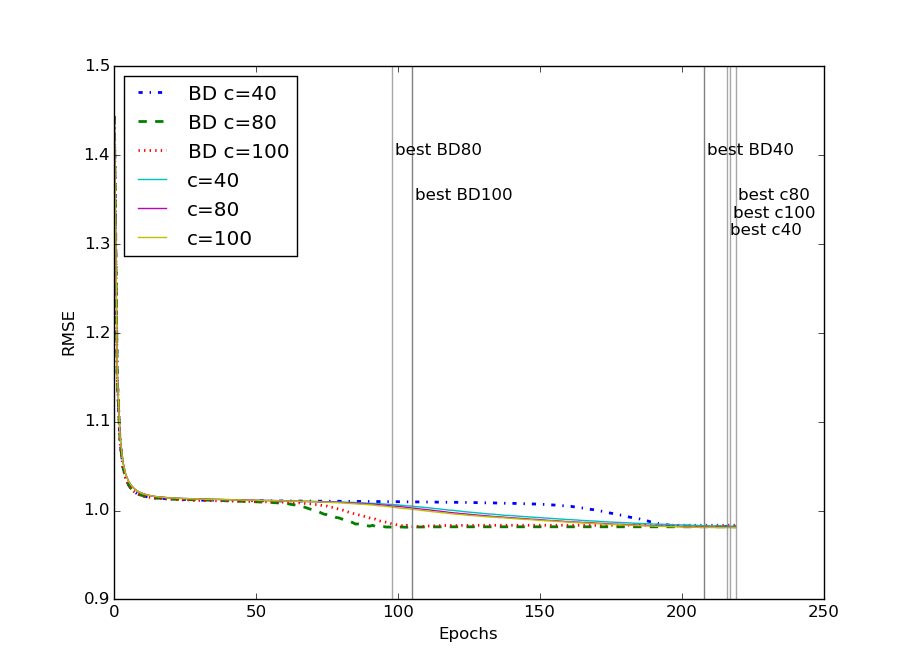
\includegraphics[scale=0.3]{convergence_speed_all.png}
		\caption{RMSE decreases with epochs for the SGD algorithm with varying $c$, with and without the bold driver heuristic. Optimal error 0.98066 was achieved after 217 epochs with C100, and 0.9811 was achieved after 98 epochs with the BD C80 setup. The vertical lines mark the epochs when the minimum error was achieved.}
		\label{fig:sgd-conv}
	\end{figure}
	
	\begin{figure}[htbp]
		\centering
		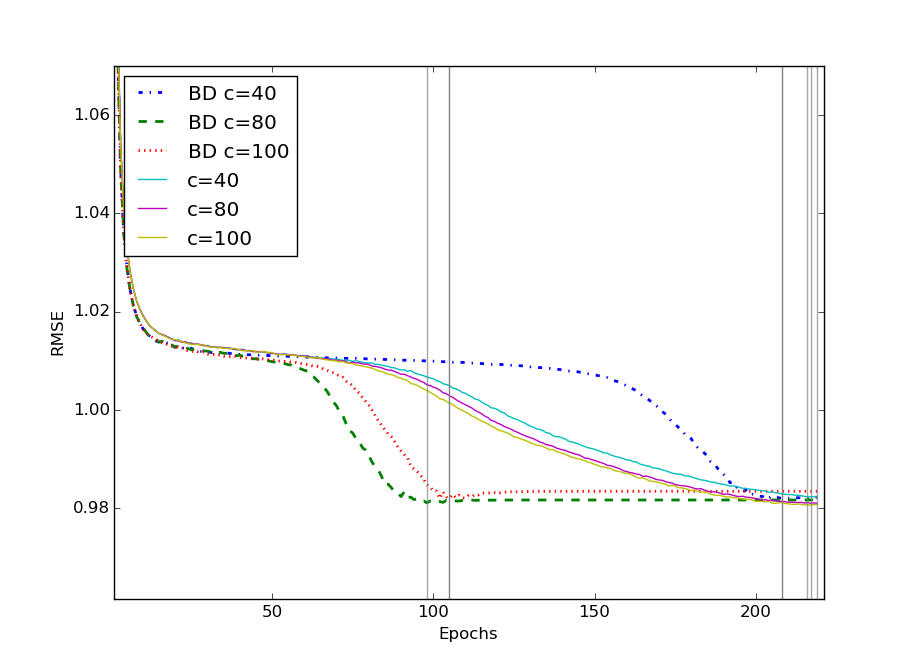
\includegraphics[scale=0.3]{convergence_zoom_all.png}
		\caption{Zoomed-in version of Figure \ref{fig:sgd-conv}. Dashed graphs show results for algorithm with bold driver heuristic. Those converge much faster than the original algorithm at the cost of a 0.0004 error increase.}
		\label{fig:sgd-conv-zoom}
	\end{figure} 
	
	\subsection{RBM Bold Driver}
	As the bold driver heuristic improved the convergence speed of SGD, we also implemented it for RBM and validated its effect. Figure \ref{fig:rbm-conv-zoom} shows how number of epochs and accuracy are affected by the bold driver heuristic. To find the optimal hyper-parameters we used \emph{grid search} on number of hidden units and learning rate, ranging between 20 and 101 and 0.03 and 0.1, respectively. The optimal error was achieved with learning rate 0.05 and 80 hidden units.
	
	
%	\begin{figure}[htbp]
%		\centering
%		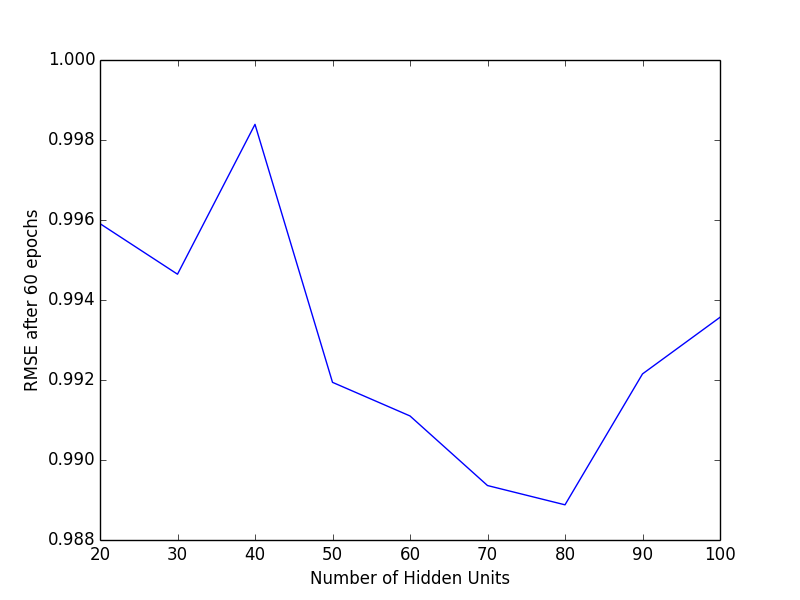
\includegraphics[width=\columnwidth]{rbm_hidden_units_effect.png}
%		\caption{Effect of number of hidden units on RMSE error of RBM, Bold driver is being used here. The errors are reported after running 60 epochs. The optimal error was achieved with 80 hidden units. }
%		\label{fig:rbm-hidden-unit}
%	\end{figure}
	
	\begin{figure}[htbp]
		\centering
		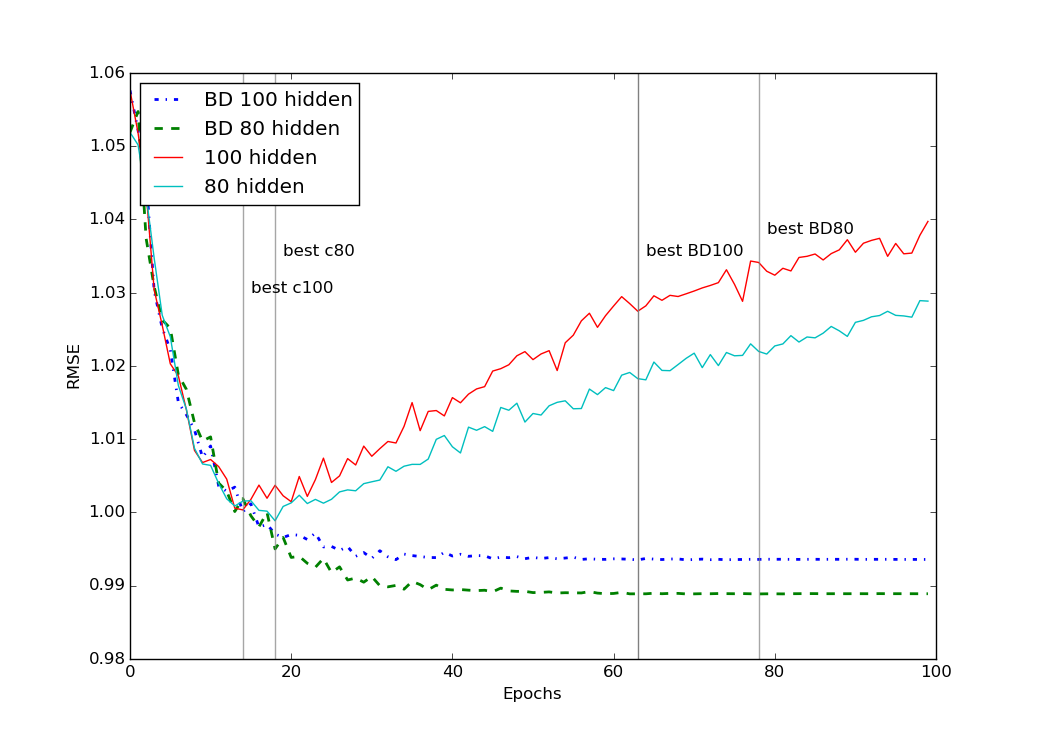
\includegraphics[scale=0.25]{conv_rbm_all.png}
		\caption{Effect of bold driver heuristic on RMSE error of RBM with 80 and 100 hidden units. The optimal error achieved without Bold Driver is 0.99883 with 100 units after 18 epochs, and 0.98885 with Bold Driver after 78 epochs.}
		\label{fig:rbm-conv-zoom}
	\end{figure} 
	
	\subsection{Comparison between baseline and optimal algorithms}
	In this section we report the RMSE error achieved on our local validation set, the public test set on Kaggle for each of the individual algorithms, and the blended result of the different algorithms.
	
	\begin{center}
		\begin{tabular}{ |p{2.8cm}||p{2.4cm}|p{2.3cm}|  }
			\hline
			Algorithm & RMSE (validation) & RMSE (Kaggle Public Testset) \\ [0.5ex] 
			\hline\hline
			SVD (K=13) & 1.00249 & 1.00082 \\ 
			\hline
			SGD (c=80) & 0.98151
			 &  0.98011 \\
			\hline
			RBM (hidden=80) & 0.98887 & 0.98814 \\
			\hline
			kNN-item (k=50) & 1.00260 & 0.99885 \\ 
			\hline
			kNN-user (k=100) & 1.00876 & 1.00569 \\ [1ex] 
			\hline
		\end{tabular}
	\end{center}
	
	We included all algorithms mentioned in the table when doing linear regression, along with some more variations. For example, we included RBM results obtained with 50 and 100 hidden states. We also included SGD results for $c = 100$. Performing linear regression on all predictions achieved a 10 fold cross validation error of 0.9420984 (Error achieved on each of the folds [0.9782558, 0.9193776, 0.94058739, 0.93060165, 0.9327, 0.98069694, 0.93532443, 0.91192913, 0.95785112, 0.93366013]). When submitting these predictions, we achieved a score of 0.96928, which outperforms each of the individual algorithms.
	
	\section{Conclusions}
	\label{sec:conclusions}
	
	The first aim of our experiments was to investigate whether we could achieve better overall accuracy by combining different algorithms which are known to perform well on the collaborative filtering problem. The intuition behind this is that different approaches to collaborative filtering capture distinct properties of the data, and so they can ``help" each other. The fact that the linear regression of predictions computed by our latent-factor and neighborhood-based algorithms outperforms all individual predictions confirms the validity of our idea.
	
	Our second contribution was investigating the bold driver heuristic. From the results of Section~\ref{sec:results}, we can easily see the positive impact of this heuristic. For SGD, adding the heuristic leads to a significant increase in convergence speed for all values of $c$ considered, especially when $c=80$ or 100 (convergence speed doubles), with very small associated error increase. The impact of the bold driver heuristic on RBM is even greater. Setups with the bold driver heuristic see their error continue to decrease for 50 or more additional epochs, achieving an improvement of 0.01 compared to the original algorithm. The difference between the behavior of the bold driver heuristic in SGD and RBM can be due to differences between the objective functions of both algorithms. It may be the case that the objective function of RBM is resistant to fixed learning rate methods, but is also well-behaved enough to be easily maneuvered by a slightly more complex method, like the bold driver.
	
%	The aim of our experiments was to investigate whether we could achieve better overall accuracy by combining different algorithms which were known to perform well on the Netflix dataset and collaborative filtering problems in general. The intuition was that latent factor models and neighbourhood based models capture different features of the underlying signal of the data. This was confirmed by bla bla bla \textbf{when we report the scores  of the pure SGD and SVD against the combination we should discuss it here}. 
%	
%	Our second contribution was investigating the bold driver heuristic. It halved the number of epochs required for the SGD algorithm to achieve the optimal values (\textbf{and RBM?} at a small cost. This was 0.0005 on the validation set, but less than \textbf{Some number here?} on the online Kaggle dataset. The convergence and accuracy of the iterative algorithm depends the C value as well, but as we can see in Figure \ref{fig:sgd-conv-zoom}, all algorithms with the Bold Driver heuristic achieve faster convergence than those without from the beginning regardless of the value of C. The Bold Driver SGD with C=40 has a later second drop (after $180^{th}$ epoch), compared to the same with $C=80$ or $100$, however it is still faster than each of the pure algorithms at the cost of $<0.001$. The effect of bold driver is even more significant on the RBM. Set-ups with the heuristic achieve a much better accuracy, as the error continues to decrease for 50 or more epochs and achieves an improvement of $0.01$ compared to the pure version. If we compare the results in Figure \ref{fig:sgd-conv-zoom} and \ref{fig:rbm-conv-zoom}, we see the differences in how the Bold Driver affects the two methods. Whereas in the case of SGD, it simply helps the algorithm to get to the optimal values faster by taking into account the curvature of the surface, in RBM it significantly improves the score. This could be due to the fact that the RBM objective function and surface are more difficult to navigate with the pure learning rate method, optimal paths can be missed and we can see that the algorithm is prone to over-fitting. The Bold Driver mitigates those dangers and is crucial to the success of the method. 
	
	
	
	
	%summarized in Table~\ref{tab:fourier-wavelet}.
	%
	%\begin{table*}[htbp]
	%  \centering
	%  \begin{tabular}[c]{|l||l|l|l|}
	%    \hline
	%    Basis&Support&Suitable signals&Unsuitable signals\\
	%    \hline
	%    Fourier&global&sine like&localized\\
	%    wavelet&local&localized&sine like\\
	%    \hline
	%  \end{tabular}
	%  \caption{Characteristics of Fourier and wavelet basis.}
	%  \label{tab:fourier-wavelet}
	%\end{table*}
	%
	%When reporting computational or measurement results, always
	%report the mean (average value) along with a measure of variability
	%(standard deviation(s) or standard error of the mean).
	
	\bibliographystyle{IEEEtran}
	\bibliography{JKM-literature}
\end{document}
